% ============================================================================
\section{Semiconductor Technology and Cell-Count Scaling}
\label{sec:semiconductor_scaling}
% ============================================================================

Semiconductor voltage scaling (Section~\ref{sec:semiconductor_limitations})
and the voltage-versus-component-count tradeoff established in
Section~\ref{sec:operating_principle} are quantified here at the
cell-count level. In an $N$-cell SPB, the dc-link voltage is
distributed among the series-connected converter cells, allowing the
use of lower-voltage semiconductor classes as $N$ increases.

The device rating must be selected from the maximum expected blocking
stress, not the nominal voltage division alone:
\begin{equation}
V_{\mathrm{rated}}
\geq
k_{\mathrm{rel}}
\left(
\frac{V_{\mathrm{dc,max}}}{N}
+\Delta V_{\mathrm{imb}}^{\max}
+\Delta V_{\mathrm{sw}}^{\max}
\right),
\label{eq:semiconductor_rating}
\end{equation}
where $\Delta V_{\mathrm{imb}}^{\max}$ denotes the maximum cell-voltage
imbalance, $\Delta V_{\mathrm{sw}}^{\max}$ the commutation overshoot,
and $k_{\mathrm{rel}}$ the selected reliability margin. Cell count is
therefore linked to discrete commercial voltage classes rather than to
a continuous semiconductor-scaling law.

As introduced in Section~\ref{sec:semiconductor_limitations}, SiC
currently provides the most direct route for high-voltage traction,
whereas GaN becomes increasingly attractive once the architecture
reduces the per-device voltage enough to access lower-voltage classes
with favorable conduction and switching characteristics
\cite{WBGTractionReview2025,Rohner2024GaN,Ebrahimian2025GaNIMMD}.

The resulting discrete design transitions are summarized and
visualized directly in Fig.~\ref{fig:cell_count_scaling}. For a
1200-V dc link, $N=2$ gives a nominal cell voltage of 600~V and
therefore leaves limited transient margin for a 650-V device.
Increasing the cell count to $N=3$ reduces the nominal cell voltage
to 400~V and provides a substantially more practical operating region
for the 650-V class. Further increases in $N$ give access to
progressively lower-voltage device families, as labeled directly on
Fig.~\ref{fig:cell_count_scaling}. The potential semiconductor benefit
is therefore nonlinear because a small change in $N$ can open a new
commercial voltage class, whereas the active-switch count grows
approximately linearly, as plotted directly from these design points
in Fig.~\ref{fig:cell_count_scaling}.

\begin{figure}[!t]
\centering
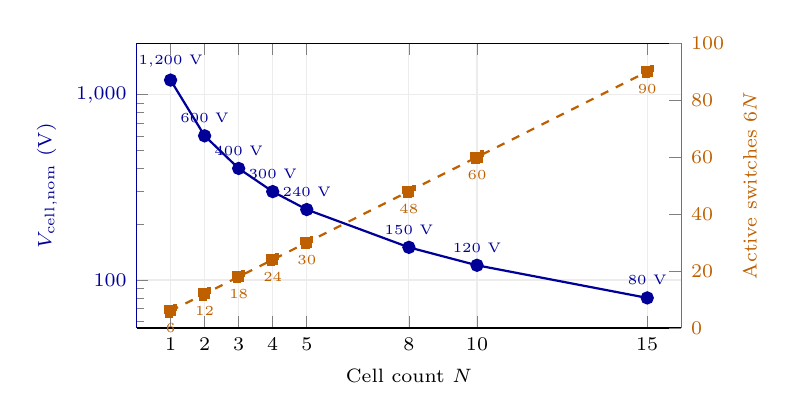
\begin{tikzpicture}
\begin{axis}[
    width=8.5cm,
    height=52mm,
    font=\scriptsize,
    xlabel={Cell count $N$},
    ylabel={$V_{\mathrm{cell,nom}}$ (V)},
    ymode=log,
    log ticks with fixed point,
    xmin=0,xmax=16,
    ymin=55,ymax=1900,
    xtick={1,2,3,4,5,8,10,15},
    axis y line*=left,
    y axis line style={draw=blue!60!black},
    tick label style={font=\scriptsize},
    yticklabel style={blue!60!black},
    xlabel style={font=\scriptsize},
    ylabel style={font=\scriptsize,blue!60!black},
    grid=major,
    grid style={gray!15},
]
\addplot[mark=*,thick,blue!60!black,
    point meta=explicit,
    nodes near coords={\pgfmathprintnumber{\pgfplotspointmeta}~V},
    every node near coord/.append style={font=\tiny,blue!60!black,anchor=south,yshift=1pt}]
    coordinates {
(1,1200)[1200](2,600)[600](3,400)[400](4,300)[300](5,240)[240]
(8,150)[150](10,120)[120](15,80)[80]};
\end{axis}
\begin{axis}[
    width=8.5cm,
    height=52mm,
    font=\scriptsize,
    xmin=0,xmax=16,
    ymin=0,ymax=100,
    xtick={1,2,3,4,5,8,10,15},
    axis x line=none,
    axis y line*=right,
    y axis line style={draw=orange!75!black},
    ylabel={Active switches $6N$},
    tick label style={font=\scriptsize},
    yticklabel style={orange!75!black},
    ylabel style={font=\scriptsize,orange!75!black},
]
\addplot[mark=square*,thick,dashed,orange!75!black,
    point meta=y,
    nodes near coords={\pgfmathprintnumber{\pgfplotspointmeta}},
    every node near coord/.append style={font=\tiny,orange!75!black,anchor=north,yshift=-1pt}]
    coordinates {
(1,6)(2,12)(3,18)(4,24)(5,30)(8,48)(10,60)(15,90)};
\end{axis}
\end{tikzpicture}
\caption{Cell-count scaling for a 1200-V dc link: nominal cell voltage
$V_{\mathrm{cell,nom}}=V_{\mathrm{dc}}/N$ (solid markers, left log
axis) and active-switch count $6N$ (dashed markers, right linear
axis) versus cell count $N$; every marker is labeled directly with
its exact value ($N=1$: 1200~V, 6; $N=2$: 600~V, 12; $N=3$: 400~V,
18; $N=4$: 300~V, 24; $N=5$: 240~V, 30; $N=8$: 150~V, 48; $N=10$:
120~V, 60; $N=15$: 80~V, 90). Increasing $N$ opens progressively lower
commercial semiconductor voltage classes (e.g., 1700--2000-V SiC at
$N=1$, 650-V GaN/SiC at $N=3$, 100-V GaN/MOSFET class at $N=15$) while
the active-switch count grows linearly as $6N$.}
\label{fig:cell_count_scaling}
\end{figure}

\subsection{Commercial-Device Screening}

Access to a lower voltage class does not by itself imply a superior
converter: the comparison must be based on commercial devices and
their conduction, switching, current, thermal, and packaging
constraints.

For nonlinear output capacitance, the stored energy
\begin{equation}
E_{\mathrm{oss}}(V)
=
\int_{0}^{V}
vC_{\mathrm{oss}}(v)\,dv
\label{eq:eoss_integral}
\end{equation}
is more informative than a single tabulated $C_{\mathrm{oss}}$ value.
Depending on the commutation process, some or all of this stored energy
can contribute to switching loss. Similarly, simple screening metrics
such as $R_{\mathrm{DS(on)}}C_{\mathrm{oss}}$ or
$R_{\mathrm{DS(on)}}Q_g$ are useful for identifying candidate devices,
but are insufficient for the final architecture comparison.

The principal device quantities required for SPB cell-count screening,
and their primary role in the comparison, are: $R_{\mathrm{DS(on)}}(T)$,
which sets the die-area or parallel-device requirement;
$E_{\mathrm{oss}}(V)$, which sets the large-signal switching penalty;
$E_{\mathrm{on/off}}(V,I,T)$, which forms the operating-point
switching-loss model; gate charge $Q_g$ and $Q_{gd}$, which govern
driver sizing and auxiliary loss; continuous current capability
$I_{\mathrm{cont}}$ and thermal resistance $R_\theta$, which govern
parallelization and cooling requirements; and package or loop
inductance $L_\sigma$, which sets the usable blocking-voltage margin
against $di/dt$-induced overshoot.

Current capability is particularly important because machine phase
current does not generally decrease in proportion to $1/N$
(Section~\ref{sec:operating_principle}). If the
derated current capability of one device is $I_{\mathrm{dev,der}}$, the
required number of parallel devices can be estimated as
\begin{equation}
n_p
=
\left\lceil
\frac{I_{\mathrm{sw,max}}}
     {I_{\mathrm{dev,der}}}
\right\rceil,
\qquad
N_{\mathrm{sw,tot}}
=
6Nn_p .
\label{eq:parallel_device_scaling}
\end{equation}
Thus, a lower-voltage device can offer an attractive device-level FOM
while still requiring substantial die area, package count, and
gate-drive/thermal interfaces. Recent high-current 650-V GaN
modules illustrate the importance of low-inductance packaging and
integrated gate driving when GaN is scaled toward traction-current
levels \cite{Zhu2024GaN150A,Rahman2025GaN300A}.

Fast switching further couples device selection to layout. The
commutation overshoot can be approximated by
\begin{equation}
\Delta V_{\mathrm{sw}}
\approx
L_{\sigma}\frac{di}{dt},
\label{eq:semiconductor_overshoot}
\end{equation}
so the benefit of reduced nominal cell voltage can be lost if package
and interconnect inductance consume a substantial fraction of the
available blocking margin. This is particularly relevant for GaN,
where high $di/dt$ places strong requirements on the commutation loop,
local decoupling, and gate-drive layout
\cite{Rahman2025GaN300A}.

GaN device selection also requires consideration of dynamic
$R_{\mathrm{DS(on)}}$, reverse conduction, gate reliability,
short-circuit capability, and thermal performance
\cite{Ajayan2025GaNReliability,Ajayan2025GaNFabrication}. These effects
do not negate the benefit of lower blocking voltage, but they prevent
room-temperature static $R_{\mathrm{DS(on)}}$ from being used as the
sole criterion for cell-count selection.

\subsection{Loss Scaling With Cell Count}

For one device, the dominant semiconductor losses can be represented
approximately as
\begin{equation}
P_{\mathrm{cond}}
\approx
I_{\mathrm{rms,sw}}^2
R_{\mathrm{DS(on)}}(T_j),
\label{eq:cond_loss_short}
\end{equation}
and
\begin{equation}
P_{\mathrm{sw}}
\approx
f_{\mathrm{sw}}
\left[
E_{\mathrm{on}}(V,I,T_j)
+
E_{\mathrm{off}}(V,I,T_j)
\right].
\label{eq:switching_loss_short}
\end{equation}

At converter level,
\begin{equation}
P_{\mathrm{semi}}(N)
=
\sum_{k=1}^{N}
\sum_{j=1}^{6n_p(N)}
\left(
P_{\mathrm{cond},k,j}
+
P_{\mathrm{sw},k,j}
+
P_{\mathrm{dt},k,j}
\right)
+
P_{\mathrm{gate}}(N).
\label{eq:complete_semiconductor_loss}
\end{equation}
The dependence on $N$ is therefore not linear. The number of active
devices increases with cell count, whereas
$R_{\mathrm{DS(on)}}$, switching energy, thermal impedance, and
parallel-device requirement can change abruptly when the design enters
a different semiconductor voltage class.

Consequently, SiC and GaN should be regarded as different regions of
the SPB design space rather than as a fixed technology ranking.
Low-cell-count architectures can favor high-voltage SiC because of its
mature voltage and current capability, whereas increasing $N$ can make
lower-voltage GaN attractive if the improvement in conduction,
switching, packaging, or passive-component performance compensates for
the additional converter modules.

Resolving the cell-count question therefore requires reading
Fig.~\ref{fig:cell_count_scaling} jointly with the screening
quantities above and the machine requirements of
Section~\ref{sec:machine_requirements}, rather than from any single
figure of merit.

